\section{HÀM SỐ BẬC NHẤT  \boldmath $y=ax+b$ ($a\ne 0$)}
\subsubsection{Kiến thức trọng tâm}
\begin{tomtat}
	\subsection{Hàm số bậc nhất, bảng giá trị}
	\begin{boxdn}
		\textbf{Hàm số bậc nhất} là hàm số cho bởi công thức $y=ax+b$, trong đó $a$, $b$ là các số cho trước và $a\ne 0$.
	\end{boxdn}
	\begin{boxdn}
		Để lập bảng giá trị của hàm số bậc nhất $y=ax+b$ ta lần lượt cho $x$ nhận các giá trị $x_{1}, x_{2}, x_{3}, \ldots$  ($x_{1}, x_{2}, x_{3}, \ldots$ tăng dần) và tính các giá trị tương ứng của $y$ rồi ghi vào bảng có dạng sau:
		\begin{center}
			\begin{tabular}{|c|c|c|c|c|}
				\hline
				$x$ & $x_{1}$ & $x_{2}$ & $x_{3}$ & $\ldots$ \\
				\hline
				$y=ax+b$ & $y_{1}$ & $y_{2}$ & $y_{3}$ & $\ldots$ \\
				\hline
			\end{tabular}
		\end{center}
	\end{boxdn}
	\subsection{Đồ thị của hàm số bậc nhất}
	\begin{boxdn}
		Đồ thị của hàm số $y=ax+b$ $(a\ne 0)$ là một đường thẳng.
	\end{boxdn}
	\begin{note}
		Đồ thị của hàm số $y=ax+b$ $(a\ne 0)$ còn được gọi là đường thẳng $y=ax+b$.
	\end{note}
	\begin{boxdn}
		\textbf{Cách vẽ đồ thị của hàm số bậc nhất}
		\immini
		{
			Ta đã biết đồ thị của hàm số bậc nhất $y=ax+b$ $(a\ne 0)$ là một đường thẳng. Do đó, để vẽ đồ thị này, ta chỉ cần xác định được hai điểm phân biệt nào đó thuộc đồ thị rồi vẽ đường thẳng đi qua hai điểm đó. Ta xét hai trường hợp:	
			\begin{itemize}
				\item Khi $b=0$ thì $y=ax$. Đồ thị của hàm số $y=ax$ là đường thẳng đi qua gốc tọa độ $O(0;0)$ và điểm $A(1;a)$ như hình bên.	
			\end{itemize}
		}
		{
			\begin{tikzpicture}[scale=1,font=\footnotesize, line join=round, line cap=round, >=stealth]
				\draw[-stealth](-1.5,0)--(2.5,0)node[below]{$x$};
				\draw[-stealth](0,-1.5)--(0,3.5)node[left]{$y$};
				\node at (0,0) [below right] {\footnotesize $O$}; 
				\draw[samples=200,domain=-.7:1.6]plot(\x,{(\x*2)});
				\draw[fill] (1,2) circle (1.5pt)node[right]{$A$}
				(1,0) node[below]{$1$}
				(0,2) node[left]{$a$}
				;
				\draw[dashed] (0,2)--(1,2)--(1,0);
			\end{tikzpicture}
		}
		\immini{
			\begin{itemize}
				\item Khi $b\ne 0$ ta thường xác định hai điểm đặc biệt trên đồ thị là giao của đồ thị với hai trục tọa độ như sau
				\begin{itemize}
					\item Cho $x=0$ thì $y=b$, ta được điểm $P(0;b)$ thuộc trục tung $Oy$.
					\item Cho $y=0$ thì $x=-\dfrac{b}{a}$, ta được điểm $Q\left(-\dfrac{b}{a};0\right)$ thuộc trục hoành $Ox$.
					\item Vẽ đường thẳng đi qua hai điểm $P$, $Q$ ta được đồ thị của hàm số $y=ax+b$ như hình bên.
				\end{itemize}	
			\end{itemize}
		}
		{
			\begin{tikzpicture}[scale=0.8,font=\footnotesize, line join=round, line cap=round, >=stealth]
				\draw[-stealth](-3.5,0)--(3.5,0)node[below]{$x$};
				\draw[-stealth](0,-2.5)--(0,3.5)node[left]{$y$};
				\node at (0,0) [below right] {\footnotesize $O$}; 
				\draw[samples=200,domain=-3.2:2.2]plot(\x,{(\x)+1});
				\draw[fill] (0,1) circle (1.5pt)node[left]{\footnotesize $P$};
				\draw[fill] (0,1) circle (1.5pt)node[right]{\footnotesize $b$};
				\draw[fill] (-1,0) circle (1.5pt)node[above left]{\footnotesize $Q$};
				\draw[fill] (-1,0) circle (1.5pt)node[below]{\footnotesize $-\dfrac{b}{a}$};
				\draw[fill] (2,2.5) node[right]{\footnotesize $y=ax+b$};
			\end{tikzpicture}	
		}
	\end{boxdn}
\end{tomtat}
%%%%%%%%%%%%

\begin{vd}%[Dự án EX-9-Đề Cương Toán 8]%[GVSB: TRẦN CHÍ VINH - GVPB1: MAI SƯƠNG - GVPB2: Nguyễn Trần Anh Tuấn]%[8D3N3-1]
	Tìm các hàm số bậc nhất trong các hàm số sau đây và chỉ ra các hệ số $a$, $b$ của các hàm số đó.
	\begin{multicols}{3}
		\begin{enumerate}
			\item $y=2 x+5$;
			\item $ y=-7$;
			\item $s=2+\dfrac{8}{x}$;
			\item $ P=9{,}8 m+2{,}3$;
			\item $ y=\sqrt{2} x+\sqrt{3}$;
			\item $ y=2 x^{2}+9.$.
		\end{enumerate}
	\end{multicols}
	\loigiai{
		\begin{enumerate}
			\item $y=2 x+5$ là hàm số bậc nhất với $a=2$ và $b=5$.
			\item $y=-7$ không là hàm số bậc nhất.
			\item $s=2+\dfrac{8}{x}$ không là hàm số bậc nhất.
			\item $P=9{,}8 m+2{,}3$ với $a=9{,}8$ và $b=2{,}3$.
			\item $ y=\sqrt{2} x+\sqrt{3}$ với $a=\sqrt{2}$ và $b=\sqrt{3}$;
			\item $ y=2 x^{2}+9.$ không là hàm số bậc nhất.
		\end{enumerate}
	}
\end{vd}
\begin{vd}%[Dự án EX-9-Đề Cương Toán 8]%[GVSB: TRẦN CHÍ VINH - GVPB1: MAI SƯƠNG - GVPB2: Nguyễn Trần Anh Tuấn]%[8D3N3-1]
	Trong các hàm số sau, hàm số nào là hàm số bậc nhất
	\begin{multicols}{3}
		\begin{enumerate}
			\item $y = 1-3x$; 
			\item $y = 2x^2 + x - 5$;
			\item $y = x^2 + x\left(\sqrt{2} - x\right) + 3$;
			\item $y = \left(\sqrt{3} - 1\right)^2x + 1$;
			\item $y=3x-2$;
			\item $y=-2x$;
			\item $y=2x^2+3$;
			\item $y=3(x-1)$;
			\item $y=0x+1$.
		\end{enumerate}
	\end{multicols}
	\loigiai{
		\begin{enumerate}
			\item Hàm số $y = 1-3x$ hay $y = -3x + 1$ có dạng $y = ax + b$, trong đó $a = -3\neq 0$, nên $y = -3x + 1$ là hàm số bậc nhất.
			\item Hàm số $y = 2x^2 + x-5$ không phải là hàm số bậc nhất vì sau khi rút gọn không có dạng $y = ax + b$.
			\item Hàm số $y = x^2 + x\left(\sqrt{2} - x\right) + 3 = x^2 + \sqrt{2}x - x^2 + 3 =\sqrt{2}x + 3$ là hàm số bậc nhất vì hàm số có dạng $y = ax + b$, trong đó $a = \sqrt{2} \neq 0$.
			\item Hàm số $y = \left(\sqrt{3} - 1\right)^2x + 1$ là hàm số bậc nhất vì hàm số có dạng $y = ax+ b$, trong đó 
			$a = \left(\sqrt{3} - 1\right)^2\neq 0$.
			\item Hàm số $y = 3x - 2$ có dạng $y = ax + b$, trong đó $a = 3 \neq 0$, nên là hàm số bậc nhất.
			\item Hàm số $y = -2x$ có dạng $y = ax + b$, trong đó $a = -2 \neq 0$, $b = 0$, nên là hàm số bậc nhất.
			\item Hàm số $y = 2x^2 + 3$ không có dạng $y = ax + b$, nên không phải là hàm số bậc nhất.
			\item Hàm số $y = 3(x - 1) = 3x - 3$ có dạng $y = ax + b$, trong đó $a = 3 \neq 0$, nên là hàm số bậc nhất.
			\item Hàm số $y = 0x + 1 = 1$ có dạng $y = b$ (hằng số), nên không phải là hàm số bậc nhất.
		\end{enumerate}
	}
\end{vd}
\begin{vd}%[Dự án EX-9-Đề Cương Toán 8]%[GVSB: TRẦN CHÍ VINH - GVPB1: MAI SƯƠNG - GVPB2: Nguyễn Trần Anh Tuấn]%[8D3H3-1]
	Tìm $m$ để các hàm số đã cho là hàm số bậc nhất.
	\begin{multicols}{2}
		\begin{enumerate}
			\item  $y = (1-2m)x + m^2 + 2$;
			\item $y = \left(m^2 - m\right) x^2 + m x + 2$
			\item $y=\left(3-2m\right)x+1$
			\item $y=(m-3)(x-1)+2$.
		\end{enumerate}
	\end{multicols}
	\loigiai{
		\begin{enumerate}
			\item Hàm số $y = (1-2m)x + m^2 + 2$ là hàm số bậc nhất khi và chỉ khi
			$1 - 2m\neq 0$ Suy ra $ m\neq\dfrac{1}{2}$.\\
			Vậy khi $ m\neq\dfrac{1}{2}$ thì hàm số $y= (1-2m)x + m^2 + 2$ là hàm số bậc nhất.
			\item 	Hàm số $y =\left(m^2 - m\right) x^2 + m x + 2$ là hàm số bậc nhất khi và chỉ khi\\
			$\heva{&m^2 - m = 0 \\& m\neq 0}$\\
			$\heva{&m(m - 1) = 0 \\&m \neq 0}$\\
			Suy ra  $m - 1 = 0$ Do đó $m = 1$.\\
			Vậy $m = 1$ thì hàm số $y =\left(m^2 - m\right) x^2 + m x + 2$ là hàm số bậc nhất.
			\item Hàm số $y=\left(3-2m\right)x+1$ là hàm số bậc nhất khi và chỉ khi $3-2m\neq 0$ Suy ra $m\neq\dfrac{3}{2}$.\\
			Vậy khi $m\neq\dfrac{3}{2}$ thì hàm số $y=\left(3-2m\right)x+1$ là hàm số bậc nhất.
			\item Hàm số $y=(m-3)(x-1)+2=(m-3)x+[\;2-(m-3)\;]$. Là bậc nhất khi\\
			$m-3\neq0\Rightarrow m\neq3$.\\
			Vậy $m\neq3$ thì hàm số $y=(m-3)(x-1)+2=(m-3)x+[\;2-(m-3)\;]$ là hàm số bậc nhất.
		\end{enumerate}
	}
\end{vd}
\begin{vd}%[Dự án EX-9-Đề Cương Toán 8]%[GVSB: TRẦN CHÍ VINH - GVPB1: MAI SƯƠNG - GVPB2: Nguyễn Trần Anh Tuấn]%[8D3N3-2]
	Lập bảng giá trị của các hàm số bậc nhất $ y=f(x)=5 x+3 \text { và } y=g(x)=-2 x+3$	
	với $x$ lần lượt bằng $-2$; $-1$; $0$; $1$; $2$.
	\loigiai{
		Bảng giá trị của hàm số $y=f(x)=5x+3$ là
		\begin{center}
			\begin{tabular}{|c|c|c|c|c|c|}
				\hline
				$x$ & $-2$ & $-1$ & $0$ & $1$ & $2$ \\
				\hline
				$y=f(x)=5 x+3$ & $-7$ & $-2$ & $3$ & $8$ & $13$ \\
				\hline
			\end{tabular}
		\end{center}
		Bảng giá trị của hàm số $y=g(x)=-2 x+3$ là 
		\begin{center}
			\begin{tabular}{|c|c|c|c|c|c|}
				\hline
				$x$ & $-2$ & $-1$ & $0$ & $1$ & $2$ \\
				\hline
				$y=g(x)=-2x+3$ & $7$ & $5$ & $3$ & $1$ & $-1$ \\
				\hline
			\end{tabular}
		\end{center}
	}	
\end{vd}
\begin{vd}%[Dự án EX-9-Đề Cương Toán 8]%[GVSB: TRẦN CHÍ VINH - GVPB1: MAI SƯƠNG - GVPB2: Nguyễn Trần Anh Tuấn]%[8D3N3-3]
	Vẽ đồ thị của các hàm số sau:
	\begin{multicols}{4}
		\begin{enumerate}
			\item $y=2 x-4$;
			\item $y=-x+3$;
			\item $y=5 x+2$;
			\item $y=-2 x-6$.
		\end{enumerate}
	\end{multicols}
	\loigiai{
		\begin{enumerate}
			\item 
			\immini{
				Với hàm số $y=2x-4$.\\
				Cho $x=0$ thì $y=-4$; \\	
				Cho $y=0$ thì $x=2$.\\	
				Đồ thị của hàm số $y=2 x-4$ là đường thẳng đi qua hai điểm $M(0 ;-4)$ và $N(2 ; 0)$.}{
				\begin{tikzpicture}[scale=0.8,font=\footnotesize, line join=round, line cap=round, >=stealth]
					\draw[-stealth](-2.5,0)--(4.5,0)node[below]{$x$};
					\draw[-stealth](0,-5)--(0,2.5)node[left]{$y$};
					\foreach \x in {-2,-1,1,2,3}{
						\fill (\x,0) node[above]{$\x$} circle(1.5pt);	}
					\foreach \y in {-4,-3,-2,-1,1,2}{
						\fill (0,\y) node[left]{$\y$} circle(1.5pt);}
					\node at (0,0) [above right] {\footnotesize $O$}; 
					\draw[samples=200,domain=-0.5:3.2]plot(\x,{2*(\x)-4});
					%	\node at (3,1) [right] {\footnot3size $B$}; 
					\draw[fill] (2,0) circle (1.5pt)node[below right]{\footnotesize $M$};
					\draw[fill] (0,-4) circle (1.5pt)node[right]{\footnotesize $N$};
					%	\draw[dashed] (2,0)--(2,-1)--(0,-1);
					%	\node at (0,-4) [right] {\footnotesize c)}; 
					%\draw[dashed] (0.5,0)--(0.5,1.25);
				\end{tikzpicture}
			}
			\item 	\immini{ Với hàm số $y=-x+3$.\\	
				Cho $x=0$ thì $y=3$;\\	
				Cho $y=0$ thì $x=3$.\\	
				Đồ thị của hàm số $y=-x+3$ là đường thẳng đi qua hai điểm $P(0 ; 3)$ và $Q(3 ; 0)$.}{
				\begin{tikzpicture}[scale=0.8,font=\footnotesize, line join=round, line cap=round, >=stealth]
					\draw[-stealth](-3.5,0)--(4.5,0)node[below]{$x$};
					\draw[-stealth](0,-2.5)--(0,4.5)node[left]{$y$};
					\foreach \x in {-2,-1,1,2,3}{
						\fill (\x,0) node[above]{$\x$} circle(1.5pt);	}
					\foreach \y in {-2,-1,1,2,3,4}{
						\fill (0,\y) node[left]{$\y$} circle(1.5pt);}
					\node at (0,0) [above right] {\footnotesize $O$}; 
					\draw[samples=200,domain=-1.2:3.9]plot(\x,{-(\x)+3});
					%	\node at (3,1) [right] {\footnot3size $B$}; 
					\draw[fill] (0,3) circle (1.5pt)node[above right]{\footnotesize $P$};
					\draw[fill] (3,0) circle (1.5pt)node[below]{\footnotesize $Q$};
					%	\draw[dashed] (2,0)--(2,-1)--(0,-1);
					%	\node at (0,-4) [right] {\footnotesize c)}; 
					%\draw[dashed] (0.5,0)--(0.5,1.25);
			\end{tikzpicture}}
			\item 
			\immini{	 Với hàm số $y=\dfrac{1}{2}x+2$.\\
				Cho $x=0$ thì $y=2$; \\	
				Cho $x=2$ thì $y=3$.\\	
				Đồ thị của hàm số $y=\dfrac{1}{2}x+2$ là đường thẳng đi qua hai điểm $M(0 ;2)$ và $N\left(2;3\right)$.}{
				\begin{tikzpicture}[scale=0.8,font=\footnotesize, line join=round, line cap=round, >=stealth]
					\draw[-stealth](-2.5,0)--(2.5,0)node[below]{$x$};
					\draw[-stealth](0,-2.5)--(0,5.0)node[left]{$y$};
					\foreach \x in {-2,-1,1,2}{
						\fill (\x,0) node[below]{$\x$} circle(1.5pt);	}
					\foreach \y in {-2,1,2,3,4}{
						\fill (0,\y) node[left]{$\y$} circle(1.5pt);}
					\node at (0,0) [above right] {\footnotesize $O$}; 
					\draw[samples=200,domain=-2.5:2.5]plot(\x,{1/2*(\x)+2});
					\draw[fill] (2,3) circle (1.5pt)node[above left]{\footnotesize $N$};
					\draw[fill] (0,2) circle (1.5pt)node[right]{\footnotesize $M$};
					\draw[dashed] (2,0)--(2,3)--(0,3);
				\end{tikzpicture}
			}
			\item 	\immini{ Với hàm số $y=-\dfrac{1}{2}x+1$.\\	
				Cho $x=0$ thì $y=1$;\\	
				Cho $x=2$ thì $y=0$.\\	
				Đồ thị của hàm số $y=-\dfrac{1}{2}x+1$ là đường thẳng đi qua hai điểm $P(0 ; 1)$ và $Q(2 ; 0)$.}{
				\begin{tikzpicture}[scale=0.8,font=\footnotesize, line join=round, line cap=round, >=stealth]
					\draw[-stealth](-3.5,0)--(4.5,0)node[below]{$x$};
					\draw[-stealth](0,-2.5)--(0,4.5)node[left]{$y$};
					\foreach \x in {-2,-1,1,2,3}{
						\fill (\x,0) node[above]{$\x$} circle(1.5pt);	}
					\foreach \y in {-2,-1,1,2,3,4}{
						\fill (0,\y) node[left]{$\y$} circle(1.5pt);}
					\node at (0,0) [above right] {\footnotesize $O$}; 
					\draw[samples=200,domain=-1.2:3.9]plot(\x,{-(\x)/2+1});
					\draw[fill] (0,1) circle (1.5pt)node[above right]{\footnotesize $P$};
					\draw[fill] (2,0) circle (1.5pt)node[below]{\footnotesize $Q$};
				\end{tikzpicture}	
			}
		\end{enumerate}
	}
\end{vd}

\subsection{Bài tập}

\begin{bt}%[Dự án EX-9-Đề Cương Toán 8]%[GVSB: TRẦN CHÍ VINH - GVPB1: MAI SƯƠNG - GVPB2: Nguyễn Trần Anh Tuấn]%[8D3N3-1]
	Tìm các hàm số bậc nhất trong các hàm số sau đây và chỉ ra các hệ số $a$, $b$ của các hàm số đó:	
	\begin{multicols}{3}
		\begin{enumerate}
			\item $y=4 x-7$;
			\item $y=x^{2}$;
			\item $y=-6 x-4$;
			\item $ y=4 x$;
			\item $y=\dfrac{3}{x}$;
			\item $ s=5 v+8$;
		\end{enumerate}
	\end{multicols}
	\loigiai{
		\begin{enumerate}
			\item Hàm số $y = 4x - 7$ có dạng $y = ax + b$, trong đó $a = 4 \neq 0$, nên $y = 4x - 7$ là hàm số bậc nhất.
			\item Hàm số $y = x^2$ không có dạng $y = ax + b$, nên không phải là hàm số bậc nhất.
			\item Hàm số $y = -6x - 4$ có dạng $y = ax + b$, trong đó $a = -6 \neq 0$, nên $y = -6x - 4$ là hàm số bậc nhất.
			\item Hàm số $y = 4x$ có dạng $y = ax + b$, trong đó $a = 4 \neq 0$, $b = 0$, nên $y = 4x$ là hàm số bậc nhất.
			\item Hàm số $y = \dfrac{3}{x}$ không có dạng $y = ax + b$, nên không phải là hàm số bậc nhất.
			\item Biểu thức $s = 5v + 8$ có dạng $s = av + b$, trong đó $a = 5 \neq 0$, nên $s = 5v + 8$ là hàm số bậc nhất theo biến $v$.
		\end{enumerate}
	}
\end{bt}
\begin{bt}%[Dự án EX-9-Đề Cương Toán 8]%[GVSB: TRẦN CHÍ VINH - GVPB1: MAI SƯƠNG - GVPB2: Nguyễn Trần Anh Tuấn]%[8D3N3-1]
	Trong các hàm số sau, những hàm số nào là hàm số bậc nhất? Hãy xác định các hệ số $a$, $b$ của chúng.
	\begin{multicols}{3}
		\begin{enumerate}
			\item $y=0x-5$;
			\item $y=1-3x$;
			\item $y=-0{,}6x$;
			\item $y=\sqrt{2}(x-1)+3$;
			\item $y=2x^2+1$;
			\item $y=-3\sqrt{x}+2$.
		\end{enumerate}
	\end{multicols}
	\loigiai{
		\begin{enumerate}
			\item Hàm số $y = 0x - 5 = -5$ có dạng $y = b$ (hằng số), không có dạng $y = ax + b$ với $a \neq 0$, nên không phải là hàm số bậc nhất.
			\item Hàm số $y = 1 - 3x = -3x + 1$ có dạng $y = ax + b$, trong đó $a = -3 \neq 0$, nên $y = -3x + 1$ là hàm số bậc nhất.
			\item Hàm số $y = -0{,}6x$ có dạng $y = ax + b$, trong đó $a = -0{,}6 \neq 0$, $b = 0$, nên $y = -0{,}6x$ là hàm số bậc nhất.
			\item Hàm số $y = \sqrt{2}(x - 1) + 3 = \sqrt{2}x - \sqrt{2} + 3 = \sqrt{2}x + (3 - \sqrt{2})$ có dạng $y = ax + b$, trong đó $a = \sqrt{2} \neq 0$, nên là hàm số bậc nhất.
			\item Hàm số $y = 2x^2 + 1$ không có dạng $y = ax + b$, nên không phải là hàm số bậc nhất.
			\item Hàm số $y = -3\sqrt{x} + 2$ không có dạng $y = ax + b$, nên không phải là hàm số bậc nhất.
		\end{enumerate}
	}
\end{bt}
\begin{bt} %[Dự án EX-9-Đề Cương Toán 8]%[GVSB: TRẦN CHÍ VINH - GVPB1: MAI SƯƠNG - GVPB2: Nguyễn Trần Anh Tuấn]%[8D3N3-1]
	Tìm các hàm số bậc nhất trong các hàm số sau đây và xác định các hệ số $a$, $b$ của chúng.
	\begin{multicols}{2}
		\begin{enumerate}
			\item $y=4 x+2$
			\item $y=5-3 x$
			\item $y=2+x^{2}$
			\item $y=-0{,}2 x$
		\end{enumerate}
	\end{multicols}
	\loigiai{
		\begin{enumerate}
			\item Hàm số $y = 4x + 2$ có dạng $y = ax + b$, trong đó $a = 4 \neq 0$, nên $y = 4x + 2$ là hàm số bậc nhất.
			\item Hàm số $y = 5 - 3x = -3x + 5$ có dạng $y = ax + b$, trong đó $a = -3 \neq 0$, nên $y = -3x + 5$ là hàm số bậc nhất.
			\item Hàm số $y = 2 + x^2 = x^2 + 2$ không có dạng $y = ax + b$, nên không phải là hàm số bậc nhất.
			\item Hàm số $y = -0{,}2x$ có dạng $y = ax + b$, trong đó $a = -0{,}2 \neq 0$, $b = 0$, nên $y = -0{,}2x$ là hàm số bậc nhất.
		\end{enumerate}
	}
\end{bt}
\begin{bt}%[Dự án EX-9-Đề Cương Toán 8]%[GVSB: TRẦN CHÍ VINH - GVPB1: MAI SƯƠNG - GVPB2: Nguyễn Trần Anh Tuấn]%[8D3H3-1]
	Tìm $m$ để các hàm số đã cho là hàm số bậc nhất.
	\begin{multicols}{2}
		\begin{enumerate}
			\item $y=(1-2m)x+m^2+5$;
			\item $y=(m^2-m)x^2+(m-2)x+1$;
			\item 	$y=(m-1) x+m$;
			\item $y=3-2 m x$;
			\item $y = m^2x + \sqrt{3} - x$;
			\item  $y = mx + 6$.
		\end{enumerate}
	\end{multicols}
	\loigiai{
		\begin{enumerate}
			\item Hàm số $y=(1-2m)x+m^2+5$ là hàm số bậc nhất khi và chỉ khỉ\\
			$1-2m\neq0$\\
			Do đó $m\neq\dfrac{1}{2}$. \\
			Vậy $m\neq\dfrac{1}{2}$ thì hàm số $y=(1-2m)x+m^2+5$ là hàm số bậc nhất.
			\item Hàm số $y=(m^2-m)x^2+(m-2)x+1$ là hàm số bậc nhất khi và chỉ khi hệ số $x^2$ bằng $0$ và hệ số $x\neq0$:\\
			Do đó $\heva{&m^2-m=0\\&m-2\neq0}$ nên $\heva{&m(m-1)=0\\&m\neq2}$.\\
			Vậy $m=0$ hoặc $m=1$ thì hàm số $y=(m^2-m)x^2+(m-2)x+1$ là hàm số bậc nhất.\\
			\item Với $m-1\ne 0$ Suy ra $m \ne 1$ thì $y=(m-1) x+m$ là hàm số bậc nhất;
			\item Với $-2m \ne 0$ Suy ra $m \ne 0$ thì $y=3-2 m x$ là hàm số bậc nhất.
			\item Ta có $y = m^2x + \sqrt{3} - x = (m^2 - 1)x + \sqrt{3}$.\\
			Để hàm số $y= (m^2 - 1)x + \sqrt{3}$ là hàm số bậc nhất thì\\
			$m^2 - 1 \neq 0$.\\
			$(m-1)(m+1)\neq0$\\
			Suy ra $m \neq 1$ và $m \neq -1$.\\
			Vậy khi $m \neq 1$ và $m \neq -1$ thì hàm số $y = m^2x + \sqrt{3} - x$ là hàm số bậc nhất.
			\item Để hàm số $y = mx + 6$ là hàm số bậc nhất thì $m\neq 0$\\
			Vậy khi $m\neq0$ thì hàm số $y = mx + 6$ là hàm số bậc nhất.
		\end{enumerate}
	}
\end{bt}
\begin{bt}%[Dự án EX-9-Đề Cương Toán 8]%[GVSB: TRẦN CHÍ VINH - GVPB1: MAI SƯƠNG - GVPB2: Nguyễn Trần Anh Tuấn]%[8D3N3-2]
	Cho hàm số bậc nhất $y=-2x+5$.
	\begin{enumerate}
		\item Hoàn thành bảng giá trị sau
		\begin{center}
			\begin{tabular}{|c|c|c|c|c|c|}
				\hline
				$x$	& $-2$ &$-1$ & $0$ &$1$ &$2$ \\
				\hline
				$y=-2x+5$	&? & ? &? & ? & ? \\
				\hline
			\end{tabular}
		\end{center}
		\item Tìm $x$ sao cho $y=12$.
	\end{enumerate}
	\loigiai{
		\begin{enumerate}
			\item Ta có bảng giá trị sau
			\begin{center}
				\begin{tabular}{|c|c|c|c|c|c|}
					\hline
					$x$	& $-2$ &$-1$ & $0$ &$1$ &$2$ \\
					\hline
					$y=-2x+5$	&$9$ & $7$ & $5$ & $3$ & $1$ \\
					\hline
				\end{tabular}
			\end{center}
			\item Ta phải tìm $x$ sao cho $y=12$, tức là $-2x+5=12$ hay $-2x=7$, suy ra $x=-\dfrac{7}{2}$.
			
		\end{enumerate}
	}
\end{bt}
\begin{bt}%[Dự án EX-9-Đề Cương Toán 8]%[GVSB: TRẦN CHÍ VINH - GVPB1: MAI SƯƠNG - GVPB2: Nguyễn Trần Anh Tuấn]%[8D3H3-2]
	Lập bảng giá trị của mỗi hàm số bậc nhất sau:
	$
	y=f(x)=4 x-1 \text { và } y=h(x)=-0{,}5 x+8
	$, với $x$ lần lượt bằng $-3$; $-2$; $-1$; $0$; $1$; $2$; $3$. Trong mỗi bảng vừa lập, khi $x$ tăng thì $y$ tăng hay giảm?
	\loigiai{
		Bảng giá trị của hàm số $y=f(x)=4x-1$ là
		\begin{center}
			\begin{tabular}{|c|c|c|c|c|c|c|c|}
				\hline
				$x$ & $-3$ & $-2$ & $-1$ & $0$ & $1$ & $2$ & $3$\\
				\hline
				$y=f(x)=4 x-1$ & $-13$ & $-9$ & $-5$ & $-1$ & $3$ & $ 7$ & $11 $ \\
				\hline
			\end{tabular}
		\end{center}
		Từ bảng giá trị ta thấy khi $x$ tăng thì $y$ tăng.\\
		Bảng giá trị của hàm số $y=h(x)=-0{,}5 x+8$ là 
		\begin{center}
			\begin{tabular}{|c|c|c|c|c|c|c|c|}
				\hline
				$x$ & $-3$ & $-2$ & $-1$ & $0$ & $1$ & $2$ & $3$\\
				\hline
				$	y=h(x)=-0{,}5 x+8 $& $9{,}5$ & $9$ & $8{,}5$ & $8$ & $7{,}5$ & $7$ & $6{,}5$ \\
				\hline
			\end{tabular}
		\end{center}
		Từ bảng giá trị ta thấy khi $x$ tăng thì $y$ giảm.\\
	}
\end{bt}
\begin{bt}%[Dự án EX-9-Đề Cương Toán 8]%[GVSB: TRẦN CHÍ VINH - GVPB1: MAI SƯƠNG - GVPB2: Nguyễn Trần Anh Tuấn]%[8D3V3-2]
	Cho hàm số bậc nhất $y=ax+3$.
	\begin{enumerate}
		\item Tìm hệ số $a$, biết rằng khi $x=1$ thì $y=5$.
		\item Với giá trị $a$ tìm được, hãy hoàn thành bảng giá trị sau vào vở:
		\begin{center}
			\begin{tabular}{|c|c|c|c|c|c|}
				\hline
				$x$	& $-2$ &$-1$ & $0$ &$1$ &$2$ \\
				\hline
				$y$	&? & ? & ? & ? & ? \\
				\hline
			\end{tabular}
		\end{center}
	\end{enumerate}
	\loigiai{
		\begin{enumerate}
			\item Thay $x=1$, $y=5$ vào hàm số $y=ax+3$, ta được 
			$a+3=5$ Suy ra $a=2$.
			\item Với giá trị $a=2$, ta có hàm số $y=2x+3$.
			\begin{center}
				\begin{tabular}{|c|c|c|c|c|c|}
					\hline
					$x$	& $-2$ &$-1$ & $0$ &$1$ &$2$ \\
					\hline
					$y=ax+3$	&$-1$ & $1$ & $3$ & $5$ & $7$ \\
					\hline
				\end{tabular}
			\end{center}
		\end{enumerate}
	}
\end{bt}
\begin{bt}%[Dự án EX-9-Đề Cương Toán 8]%[GVSB: TRẦN CHÍ VINH - GVPB1: MAI SƯƠNG - GVPB2: Nguyễn Trần Anh Tuấn]%[8D3N3-3]
	Vẽ đồ thị của các hàm số sau
	\begin{multicols}{3}
		\begin{enumerate}
			\item $y=2x-6$;
			\item $y=-3x+5$;
			\item $y=\dfrac{3}{2}x$;
			\item $y=3 x$;
			\item $y=\dfrac{1}{3} x$;
			\item $y=2x+4$.
		\end{enumerate}
	\end{multicols}
	\loigiai{
		\begin{enumerate}
			\item \immini{
				Vẽ đồ thị hàm số $y=2x+6$.\\	 
				Cho $x=0$ thì $y=6$, ta được giao điểm của đồ thị với trục $Oy$ là $P(0;6)$. \\	
				Cho $y=0$ thì $x=-3$, ta được giao điểm của đồ thị với trục $Ox$ là $Q\left(-3;0\right)$.\\	
				Đồ thị của hàm số $y=2x+6$ là đường thẳng $PQ$.}{
				\begin{tikzpicture}[scale=0.8,font=\footnotesize, line join=round, line cap=round, >=stealth]
					\draw[-stealth](-3.5,0)--(3.5,0)node[below]{$x$};
					\draw[-stealth](0,-1.5)--(0,7.5)node[left]{$y$};
					\foreach \x in {-3,-2,-1,1,2}{
						\fill (\x,0) node[below]{$\x$} circle(1pt);	}
					\foreach \y in {-1,1,2,3,4,5,6}{
						\fill (0,\y) node[left]{$\y$} circle(1pt);}
					\node at (0,0) [below right] {\footnotesize $O$}; 
					\draw[samples=200,domain=-3.5:.5]plot(\x,{2*(\x)+6});
					\draw[fill] (0,6) circle (1.5pt)node[right]{$P$};
					\draw[fill] (-3,0) circle (1.5pt)node[above left]{$Q$};
				\end{tikzpicture}
			}	
			\item \immini{
				Vẽ đồ thị hàm số $y=-3x+5$.\\	 
				Cho $x=0$ thì $y=5$, ta được giao điểm của đồ thị với trục $Oy$ là $P(0;6)$. \\	
				Cho $x=1$ thì $y=2$, ta được điểm $Q\left(1;2\right)$.\\	
				Đồ thị của hàm số $y=-3x+5$ là đường thẳng $PQ$. }{
				\begin{tikzpicture}[scale=0.8,font=\footnotesize, line join=round, line cap=round, >=stealth]
					\draw[-stealth](-3.5,0)--(3.5,0)node[below]{$x$};
					\draw[-stealth](0,-1.5)--(0,6.5)node[left]{$y$};
					\foreach \x in {-3,-2,-1,1,2,3}{
						\fill (\x,0) node[below]{$\x$} circle(1pt);	}
					\foreach \y in {-1,1,2,3,4,5}{
						\fill (0,\y) node[left]{$\y$} circle(1pt);}
					\node at (0,0) [below right] {\footnotesize $O$}; 
					\draw[samples=200,domain=-.5:2]plot(\x,{-3*(\x)+5});
					\draw[fill] (0,5) circle (1.5pt)node[right]{$P$};
					\draw[fill] (1,2) circle (1.5pt)node[above right]{$Q$};
					\draw[dashed] (0,2)--(1,2)--(1,0);
				\end{tikzpicture}
			}	
			\item \immini{
				Vẽ đồ thị hàm số $y=\dfrac{3}{2}x$.\\	 
				Cho $x=0$ thì $y=0$, ta được điểm $O(0;0)$. \\	
				Cho $x=2$ thì $y=3$, ta được điểm $A(2;3)$.\\	
				Đồ thị của hàm số $y=\dfrac{3}{2}x$ là đường thẳng $OA$.}{
				\begin{tikzpicture}[scale=0.8,font=\footnotesize, line join=round, line cap=round, >=stealth]
					\draw[-stealth](-3.5,0)--(3.5,0)node[below]{$x$};
					\draw[-stealth](0,-1.5)--(0,3.5)node[left]{$y$};
					\foreach \x in {-2,-1,1,2,3}{
						\fill (\x,0) node[below]{$\x$} circle(1pt);	}
					\foreach \y in {-1,1,2,3}{
						\fill (0,\y) node[left]{$\y$} circle(1pt);}
					\node at (0,0) [below right] {\footnotesize $O$}; 
					\draw[samples=200,domain=-1:2.2]plot(\x,{1.5*(\x)});
					\draw[fill] (2,3) circle (1.5pt)node[above left]{$A$};
					%	\draw[fill] (-2,0) circle (1pt)node[below right]{$-2$};
					\draw[dashed] (0,3)--(2,3)--(2,0);
				\end{tikzpicture}
			}
			\item \immini{Cho $x=1$ ta có $y=3$. Ta vẽ điểm $A(1 ; 3)$. Đồ thị hàm số $y=3 x$ là đường thẳng đi qua các điểm $O(0 ; 0)$ và $A(1 ; 3)$ }{		\begin{tikzpicture}[scale=0.8,font=\footnotesize, line join=round, line cap=round, >=stealth]
					\draw[-stealth](-3.5,0)--(3.5,0)node[below]{$x$};
					\draw[-stealth](0,-3.5)--(0,3.5)node[left]{$y$};
					\foreach \x in {-3,-2,-1,1,2,3}{
						\fill (\x,0) node[below]{$\x$} circle(1.5pt);	}
					\foreach \y in {-3,-2,-1,1,2,3}{
						\fill (0,\y) node[left]{$\y$} circle(1.5pt);}
					\node at (0,0) [below right] {\footnotesize $O$}; 
					\draw[samples=200,domain=-1.2:1.2]plot(\x,{3*(\x)});
					\draw[fill] (1,3) circle (1.5pt)node[right]{\footnotesize $A$};
					\draw[dashed] (1,0)--(1,3)--(0,3);
					%\draw[dashed] (0.5,0)--(0.5,1.25);
			\end{tikzpicture}}
			\item \immini{Cho $x=3$ ta có $y=1$. Ta vẽ điểm $B(3 ; 1)$. Đồ thị hàm số $y=\dfrac{1}{3} x$ là đường thẳng đi qua các điểm $O(0 ; 0)$ và $B(3 ; 1)$.}{		\begin{tikzpicture}[scale=0.8,font=\footnotesize, line join=round, line cap=round, >=stealth]
					\draw[-stealth](-3.5,0)--(3.5,0)node[below]{$x$};
					\draw[-stealth](0,-2.5)--(0,2.5)node[left]{$y$};
					\foreach \x in {-3,-2,-1,1,2,3}{
						\fill (\x,0) node[below]{$\x$} circle(1.5pt);	}
					\foreach \y in {-2,-1,1,2}{
						\fill (0,\y) node[left]{$\y$} circle(1.5pt);}
					\node at (0,0) [below right] {\footnotesize $O$}; 
					\draw[samples=200,domain=-3.2:3.2]plot(\x,{0.3333*(\x)});
					%	\node at (3,1) [right] {\footnotesize $B$}; 
					\draw[fill] (3,1) circle (1.5pt)node[right]{\footnotesize $B$};
					\draw[dashed] (3,0)--(3,1)--(0,1);
					%\draw[dashed] (0.5,0)--(0.5,1.25);
			\end{tikzpicture}}
			\item	 
			\immini{Cho $x=0$ thì $y=4$, ta được giao điểm của đồ thị với trục $Oy$ là $P(0;4)$. \\	
				Cho $y=0$ thì $x=-2$, ta được giao điểm của đồ thị với trục $Ox$ là $Q(-2;0)$.\\	
				Đồ thị của hàm số $y=2x+4$ là đường thẳng $PQ$.}{
				\begin{tikzpicture}[scale=1,font=\footnotesize, line join=round, line cap=round, >=stealth]
					\draw[-stealth](-3.5,0)--(3.5,0)node[below]{$x$};
					\draw[-stealth](0,-1.5)--(0,5.5)node[left]{$y$};
					\foreach \x in {-3,-1,1,2,3}{
						\fill (\x,0) node[below]{$\x$} circle(1pt);	}
					\foreach \y in {-1,1,2,3,4,5}{
						\fill (0,\y) node[left]{$\y$} circle(1pt);}
					\node at (0,0) [below right] {\footnotesize $O$}; 
					\draw[samples=200,domain=-2.5:.5]plot(\x,{2*(\x)+4});
					\draw[fill] (0,4) circle (1.5pt)node[right]{$P$};
					\draw[fill] (-2,0) circle (1.5pt)node[above left]{$Q$};
					\draw[fill] (-2,0) circle (1pt)node[below right]{$-2$};
				\end{tikzpicture}
			}
		\end{enumerate}	
	}
\end{bt}
\begin{bt}%[Dự án EX-9-Đề Cương Toán 8]%[GVSB: TRẦN CHÍ VINH - GVPB1: MAI SƯƠNG - GVPB2: Nguyễn Trần Anh Tuấn]%[8D3N3-3]
	Vẽ đồ thị của các hàm số bậc nhất $y=-2x+3$ và $y=\dfrac{1}{2}x$.
	\loigiai{
		\immini{
			\textbf{Vẽ đồ thị hàm số $y=-2x+3$.}\\	 
			Cho $x=0$ thì $y=3$, ta được giao điểm của đồ thị với trục $Oy$ là $P(0;3)$. \\	
			Cho $y=0$ thì $x=\dfrac{3}{2}$, ta được giao điểm của đồ thị với trục $Ox$ là $Q\left(\dfrac{3}{2};0\right)$.\\	
			Đồ thị của hàm số $y=-2x+3$ là đường thẳng $PQ$.}{
			\begin{tikzpicture}[scale=1,font=\footnotesize, line join=round, line cap=round, >=stealth]
				\draw[-stealth](-3.5,0)--(3.5,0)node[below]{$x$};
				\draw[-stealth](0,-1.5)--(0,5.5)node[left]{$y$};
				\foreach \x in {-2,-1,1,2,3}{
					\fill (\x,0) node[below]{$\x$} circle(1pt);	}
				\foreach \y in {-1,1,2,3,4,5}{
					\fill (0,\y) node[left]{$\y$} circle(1pt);}
				\node at (0,0) [below right] {\footnotesize $O$}; 
				\draw[samples=200,domain=-1:2]plot(\x,{-2*(\x)+3});
				\draw[fill] (0,3) circle (1.5pt)node[right]{$P$};
				\draw[fill] (1.5,0) circle (1.5pt)node[above right]{$Q$};
			\end{tikzpicture}
		}	
		\immini{
			\textbf{Vẽ đồ thị hàm số $y=\dfrac{1}{2}x$.}\\	 
			Cho $x=0$ thì $y=0$, ta được điểm $O(0;0)$. \\	
			Cho $x=2$ thì $y=1$, ta được điểm $A(2;1)$.\\	
			Đồ thị của hàm số $y=\dfrac{1}{2}x$ là đường thẳng $OA$.}{
			\begin{tikzpicture}[scale=1,font=\footnotesize, line join=round, line cap=round, >=stealth]
				\draw[-stealth](-3.5,0)--(3.5,0)node[below]{$x$};
				\draw[-stealth](0,-1.5)--(0,3.5)node[left]{$y$};
				\foreach \x in {-2,-1,1,2,3}{
					\fill (\x,0) node[below]{$\x$} circle(1pt);	}
				\foreach \y in {-1,1,2,3}{
					\fill (0,\y) node[left]{$\y$} circle(1pt);}
				\node at (0,0) [below right] {\footnotesize $O$}; 
				\draw[samples=200,domain=-2.5:3]plot(\x,{.5*(\x)});
				\draw[fill] (2,1) circle (1.5pt)node[above]{$A$};
				%	\draw[fill] (-2,0) circle (1pt)node[below right]{$-2$};
				\draw[dashed] (0,1)--(2,1)--(2,0);
			\end{tikzpicture}
		}	
	}
\end{bt}%[Dự án EX-9-Đề Cương Toán 8]%[GVSB: TRẦN CHÍ VINH - GVPB1: MAI SƯƠNG - GVPB2: Nguyễn Trần Anh Tuấn]%[8D3H3-3]
\begin{bt} Cho các hàm số $y=x$; $y=x+2$; $y=-x$; $y=-x+2$
	\begin{enumerate}
		\item Vẽ đồ thị các hàm số đã cho trên cùng một mặt phẳng toạ độ.
		\item Bốn đồ thị nói trên cắt nhau tại các điểm $O(0; 0)$, $A$, $B$, $C$. Tứ giác có $4$ đỉnh $O$, $A$, $B$, $C$ là hình gì? Giải thích.
	\end{enumerate}
	\loigiai{
		\begin{enumerate}
			\item 			
			\begin{itemize}
				\item Với hàm số $y=x$.\\
				Cho $x=1$ thì $y=1$. \\	
				Đồ thị của hàm số $y= x$ là đường thẳng đi qua hai điểm $O(0 ;0)$ và $C\left(1;1\right)$.
				\item Với hàm số $y=-x$.\\
				Cho $x=-1$ thì $y=1$. \\	
				Đồ thị của hàm số $y= -x$ là đường thẳng đi qua hai điểm $O(0 ;0)$ và $A\left(-1;1\right)$.
				\item Với hàm số $y=x+2$.\\
				Cho $x=0$ thì $y=2$; \\	
				Cho $x=-2$ thì $y=0$. \\	
				Đồ thị của hàm số $y= x+2$ là đường thẳng đi qua hai điểm $B(0 ;2)$ và $N\left(-2;0\right)$.
				\item Với hàm số $y=-x+2$.\\
				Cho $x=0$ thì $y=2$; \\	
				Cho $x=2$ thì $y=0$. \\	
				Đồ thị của hàm số $y= x$ là đường thẳng đi qua hai điểm $B(0 ;2)$ và $Q\left(2;0\right)$.
			\end{itemize}
			\begin{center}
				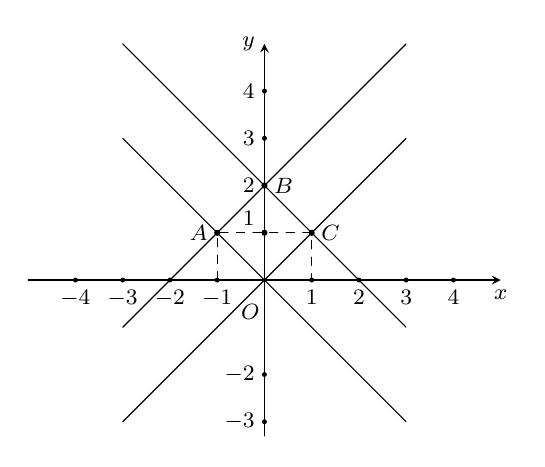
\begin{tikzpicture}[scale=0.6,font=\footnotesize, line join=round, line cap=round, >=stealth]
					\draw[-stealth](-5,0)--(5,0)node[below]{$x$};
					\draw[-stealth](0,-3.3)--(0,5.0)node[left]{$y$};
					\foreach \x in {-4,-3,-2,-1,1,2,3,4}{
						\fill (\x,0) node[below]{$\x$} circle(1.5pt);	}
					\foreach \y in {-3,-2,2,3,4}{
						\fill (0,\y) node[left]{$\y$} circle(1.5pt);}
					\node at (-0.3,-0.3) [below] { \small \footnotesize $O$}; 
					\draw[samples=200,domain=-3:3]plot(\x,{(\x)});
					\draw[samples=200,domain=-3:3]plot(\x,{-(\x)});
					\draw[samples=200,domain=-3:3]plot(\x,{(\x)+2});
					\draw[samples=200,domain=-3:3]plot(\x,{-(\x)+2});
					%	\node at (3,1) [right] {\footnot3size $B$}; 
					\draw[fill] (1,1) circle (1.5pt)node[right]{\footnotesize $C$};
					\draw[fill] (-1,1) circle (1.5pt)node[left]{\footnotesize $A$};
					\draw[fill] (0,2) circle (1.5pt)node[right]{\footnotesize $B$};
					\draw[fill] (0,1) circle (1.5pt);
					\draw[fill] (0,1.3) node[left]{$1$};
					\draw[dashed] (-1,0)--(-1,1)--(1,1)--(1,0);
					%	\node at (0,-4) [right] {\footnotesize c)}; 
					%\draw[dashed] (0.5,0)--(0.5,1.25);
				\end{tikzpicture}
			\end{center}	
			\item Dựa vào đồ thị trên ta có các điểm $O(0; 0), ~A(-1,1), ~B(0,2), ~C(1,1)$. Do đó $OB$ và $AC$ vuông góc và cắt nhau tại trung điểm mỗi đường là $I(0,1)$, ngoài ra ta có $OB=AC=2$. Suy ra $OABC$ là hình vuông (dấu hiệu nhận biết hình vuông).
		\end{enumerate}
		
	} 
\end{bt}
\begin{bt}%[Dự án EX-9-Đề Cương Toán 8]%[GVSB: TRẦN CHÍ VINH - GVPB1: MAI SƯƠNG - GVPB2: Nguyễn Trần Anh Tuấn]%[8D3N3-4]
	Để đổi nhiệt độ từ độ $F$ (Fahrenheit) sang độ $C$ (Celsius), ta dùng công thức $C=\dfrac{5}{9}(F-32)$.
	\begin{enumerate}
		\item $C$ có phải là hàm số bậc nhất theo biến số $F$ không?
		\item Hãy tính $C$ khi $F=32$ và tính $F$ khi $C=100$.
	\end{enumerate}
	\loigiai{
		\begin{enumerate}
			\item Ta có $C=\dfrac{5}{9}(F-32) = \dfrac{5}{9}F - \dfrac{160}{9}$.\\
			Do đó $C$ là hàm số bậc nhất theo biến $F$ với $a=\dfrac{5}{9}$ và $b=- \dfrac{160}{9}$.
			\item $F=32 \Rightarrow C = \dfrac{5}{9}(32-32)=0$.\\
			$C=100 \Rightarrow 100 = \dfrac{5}{9}(F-32)=0 \Leftrightarrow F = 212$.
		\end{enumerate}
	}
\end{bt}
\begin{bt}%[Dự án EX-9-Đề Cương Toán 8]%[GVSB: TRẦN CHÍ VINH - GVPB1: MAI SƯƠNG - GVPB2: Nguyễn Trần Anh Tuấn]%[8D3H3-4]
	Gọi $C$ và $r$ lần lượt là chu vi và bán kính của một đường tròn. Hãy chứng tỏ $C$ là một hàm số bậc nhất theo biến số $r$. Tìm hệ số $a$, $b$ của hàm số này.
	\loigiai{
		Theo công thức tính chu vi đường tròn ta có $C=2\pi r$.\\ 
		Do đó $C$ là hàm số bậc nhất theo biến số $r$ với $a=2\pi$ và $b=0$.	
	}
\end{bt}
\begin{bt}%[Dự án EX-9-Đề Cương Toán 8]%[GVSB: TRẦN CHÍ VINH - GVPB1: MAI SƯƠNG - GVPB2: Nguyễn Trần Anh Tuấn]%[8D3H3-4]
	Một người đi bộ trên đường thẳng với tốc độ $v~(\mathrm{km} / \mathrm{h})$.
	Gọi $s~(\mathrm{km})$ là quãng đường đi được trong $t$ (giờ).
	\begin{enumerate}
		\item Lập công thức tính $s$ theo $t$.
		\item Vẽ đồ thị của hàm số $s$ theo biến số $t$ khi $v=4$.
	\end{enumerate}
	\loigiai{\immini{
			\begin{enumerate}
				\item Theo công thức tính quãng đường theo vận tốc và thời gian ta có $s=vt$.
				\item Khi $v=4$, ta có $s=4t$, trong đó $t \ge 0$.\\
				Cho $t=1$ thì $y=4$. \\	
				Đồ thị của hàm số $s= 4t$ là đường thẳng đi qua hai điểm $O(0 ;0)$ và $A\left(1;4\right)$.
			\end{enumerate}
		}{
			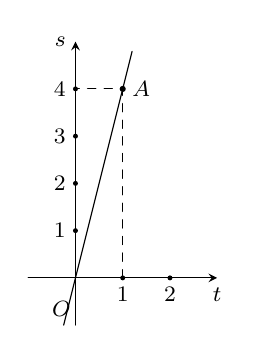
\begin{tikzpicture}[scale=0.6,font=\footnotesize, line join=round, line cap=round, >=stealth]
				\draw[-stealth](-1,0)--(3,0)node[below]{$t$};
				\draw[-stealth](0,-1)--(0,5.0)node[left]{$s$};
				\foreach \x in {1,2}{
					\fill (\x,0) node[below]{$\x$} circle(1.5pt);	}
				\foreach \y in {1,2,3,4}{
					\fill (0,\y) node[left]{$\y$} circle(1.5pt);}
				\node at (-0.3,-0.3) [below] { \small \footnotesize $O$}; 
				\draw[samples=200,domain=-0.25:1.2]plot(\x,{4*(\x)});
				\draw[fill] (1,4) circle (1.5pt)node[right]{\footnotesize $A$};
				\draw[dashed] (1,0)--(1,4)--(0,4);
			\end{tikzpicture}
		}
	}
\end{bt}
\begin{bt}%[Dự án EX-9-Đề Cương Toán 8]%[GVSB: TRẦN CHÍ VINH - GVPB1: MAI SƯƠNG - GVPB2: Nguyễn Trần Anh Tuấn]%[8D3H3-4]
	Đồng euro (EUR) là đơn vị tiền tệ chính thức ở một số quốc gia thành viên của Liên minh châu Âu. Vào một ngày, tỉ giá hối đoái giữa đồng euro và đồng đô la Mỹ (USD) là $1$ EUR $=1{,}1052$ USD.
	\begin{enumerate}
		\item Viết công thức để chuyển đổi $x$ euro sang $y$ đô la Mỹ. Công thức tính $y$ theo $x$ này có phải là một hàm số bậc nhất của $x$ không?
		\item Vào ngày đó, $200$ euro có giá trị bằng bao nhiêu đô la Mỹ?
		\item Vào ngày đó, $500$ đô la Mỹ có giá trị bằng bao nhiêu euro?
	\end{enumerate}
	\loigiai{
		\begin{enumerate}
			\item Công thức để chuyển đổi $x$ euro sang $y$ đô la Mỹ là $y=1,1052x$.\\
			Công thức tính $y$ theo $x$ này là một hàm số bậc nhất của $x$. 
			\item $200$ euro có giá trị là $1,1052\cdot 200=210,4$ đô la Mỹ.
			\item $500$ đô la Mỹ có giá trị là $500:1,1052\approx 475,3$ euro.
		\end{enumerate}
	}
\end{bt}
\begin{bt}%[Dự án EX-9-Đề Cương Toán 8]%[GVSB: TRẦN CHÍ VINH - GVPB1: MAI SƯƠNG - GVPB2: Nguyễn Trần Anh Tuấn]%[8D3H3-4]
	Giá cước điện thoại cố định của một hãng viễn thông bao gồm cước thuê bao là $22\,000$ đồng/tháng và cước gọi là $800$ đồng/phút.
	\begin{enumerate}
		\item Lập công thức tính số tiền cước điện thoại $y$ (đồng) phải trả trong tháng khi gọi $x$ phút.
		\item Tính số tiền cước điện thoại phải trả khi gọi $75$ phút.
		\item Nếu số tiền cước điện thoại phải trả là $94\,000$ đồng thì trong tháng đó thuê bao đã gọi bao nhiêu phút?
	\end{enumerate}
	\loigiai{
		\begin{enumerate}
			\item Công thức tính số tiền cước điện thoại $y$ (đồng) phải trả trong tháng khi gọi $x$ phút là\\ 
			$y=800x+22\,000$.
			\item Số tiền cước điện thoại phải trả khi gọi $75$ phút là\\ $800\cdot 75+22\,000=82\,000$ (đồng).
			\item Thay $y=94\,000$ vào $y=800x+22\,000$, ta được\\
			$800x+22\,000=94\,000\Rightarrow x=90$.\\
			Vậy nếu số tiền cước điện thoại phải trả là $94\,000$ đồng thì trong tháng đó thuê bao đã gọi $90$ phút.
		\end{enumerate}
	}
\end{bt}
\begin{bt}%[Dự án EX-9-Đề Cương Toán 8]%[GVSB: TRẦN CHÍ VINH - GVPB1: MAI SƯƠNG - GVPB2: Nguyễn Trần Anh Tuấn]%[8D3H3-4]
	Hàm chi phí đơn giản nhất là hàm chi phí bậc nhất $y=ax+b$, trong đó $b$ biểu thị chi phí cố định của hoạt động kinh doanh và hệ số $a$ biểu thị chi phí của mỗi mặt hàng được sản xuất. Giả sử rằng một xưởng sản xuất xe đạp có chi phí cố định hằng ngày là $36$ triệu đồng và mỗi chiếc xe đạp có chi phí sản xuất là $1,8$ triệu đồng.
	\begin{enumerate}
		\item Viết công thức của hàm số bậc nhất biểu thị chi phí $y$ (triệu đồng) để sản xuất $x$ (xe đạp) trong một ngày.
		\item Vẽ đồ thị của hàm số thu được ở câu $a$.
		\item Chi phí để sản xuất $15$ chiếc xe đạp trong một ngày là bao nhiêu?
		\item Có thể sản xuất bao nhiêu chiếc xe đạp trong ngày, nếu chi phí trong ngày đó là $72$ triệu đồng?
	\end{enumerate}
	
	\loigiai{
		\begin{enumerate}
			\item Công thức của hàm số bậc nhất biểu thị chi phí $y$ (triệu đồng) để sản xuất $x$ (xe đạp) trong một ngày là
			$$y=1{,}8x+36.$$
			\item 
			\immini{
				\textbf{ Vẽ đồ thị hàm số $y=1{,}8x+36$.}\\	 
				Cho $x=0$ thì $y=36$, ta được điểm $A(0;36)$. \\	
				Cho $y=0$ thì $y=-20$, ta được điểm $B(-20;0)$.\\	
				Đồ thị của hàm số $y=1{,}8x+36$ là đường thẳng $AB$.}
			{
				\begin{tikzpicture}[scale=1,font=\footnotesize, line join=round, line cap=round, >=stealth]
					\draw[-stealth](-3.5,0)--(3.5,0)node[below]{$x$};
					\draw[-stealth](0,-1.5)--(0,4.5)node[left]{$y$};
					\foreach \x in {-30,-20,-10,10,20,30}{
						\fill (\x/10,0) node[below]{$\x$} circle(1pt);	}
					\foreach \y in {-10,10,20,30,40}{
						\fill (0,\y/10) node[left]{$\y$} circle(1pt);}
					\node at (0,0) [below right] {\footnotesize $O$}; 
					\draw[fill] (0,3.6) circle (1.5pt)node[above right]{$A$};
					\draw[fill] (-2,0) circle (1.5pt)node[above left]{$B$};
					\path
					(0,3.6) coordinate (A)
					(-2,0) coordinate (B)
					($(A)!1.2!(B)$) coordinate (M)
					($(A)!-.2!(B)$) coordinate(N)
					;
					\draw (M)--(N);
				\end{tikzpicture}
			}
			\item Chi phí để sản xuất $15$ chiếc xe đạp trong một ngày là 
			$$1,8\cdot 15+36=63~\text{ (triệu đồng).}$$
			\item Thay $y=72$ vào hàm số $y=1{,}8x+36$, ta được
			$$1{,}8x+36=72\Rightarrow x=20.$$
			Vậy nếu chi phí trong ngày đó là $72$ triệu đồng thì có thể sản xuất $20$ chiếc xe đạp trong ngày.
		\end{enumerate}
	}
\end{bt}
\begin{bt}%[Dự án EX-9-Đề Cương Toán 8]%[GVSB: TRẦN CHÍ VINH - GVPB1: MAI SƯƠNG - GVPB2: Nguyễn Trần Anh Tuấn]%[8D3V3-4]
	\immini{
		Một lò xo có chiều dài ban đầu khi chưa treo vật nặng là $10 \mathrm{~cm}$. Cho biết khi treo thêm vào lò xo một vật nặng $1 \mathrm{~kg}$ thì chiều dài lò xo tăng thêm $3 \mathrm{~cm}$.
		\begin{enumerate}
			\item Tính chiều dài $y~(\mathrm{cm})$ của lò xo theo khối lượng $x~(\mathrm{kg})$ của vật.
			\item Vẽ đồ thị của hàm số $y$ theo biến số $x$.
		\end{enumerate}
	}{
		\begin{tikzpicture}
			\node[circle,fill=blue,inner sep=0.5mm] (b) at (2,2) {};
			\draw[decoration={aspect=0.3, segment length=1.5mm, amplitude=3mm,coil},decorate] (2,5) -- (b); 
			\fill [pattern = north east lines] (1.2,5) rectangle (3,5.2);
			\draw[thick] (1.2,5) -- (3,5);
			\draw[dashed] (2.5,5) -- (3.5,5);
			\draw[dashed] (2.5,2) -- (3.5,2);
			\draw[latex-latex] (3,5) -- node[right=0.1cm]{$10$ cm} (3,2); 
		\end{tikzpicture}
	}
	\loigiai{
		\begin{center}
			\begin{tikzpicture}
				\node[circle,fill=blue,inner sep=0.5mm] (a) at (0,0) { \textcolor{white}{$x$ kg}};
				\node[circle,fill=blue,inner sep=0.5mm] (b) at (2,2) {};
				\draw[decoration={aspect=0.3, segment length=3mm, amplitude=3mm,coil},decorate] (0,5) -- (a); 
				\draw[decoration={aspect=0.3, segment length=1.5mm, amplitude=3mm,coil},decorate] (2,5) -- (b); 
				\fill [pattern = north east lines] (-1,5) rectangle (1,5.2);
				\fill [pattern = north east lines] (1.2,5) rectangle (3,5.2);
				\draw[thick] (-1,5) -- (1,5);
				\draw[thick] (1.2,5) -- (3,5);
				\draw[dashed] (0.5,0) -- (1.5,0);
				\draw[dashed] (0.5,2) -- (1.5,2);
				\draw[latex-latex] (1,0) -- node[right=0.1cm]{$3x$ cm} (1,2); 
				\draw[dashed] (2.5,5) -- (3.5,5);
				\draw[dashed] (2.5,2) -- (3.5,2);
				\draw[latex-latex] (3,5) -- node[right=0.1cm]{$10$ cm} (3,2); 
			\end{tikzpicture}
		\end{center}
		\immini{
			\begin{enumerate}
				\item Chiều dài của lò xo tăng thêm khi treo vật có khối lượng $x~(\mathrm{kg})$ là $3x$. Vậy $y=3x+10$ (cm).
				\item 	Cho $x=0$ thì $y=10$;\\	
				Cho $y=0$ thì $x=-\dfrac{10}{3}$.\\	
				Đồ thị của hàm số $y=3x+10$ là đường thẳng đi qua hai điểm $A(0 ; 10)$ và $B\left(-\dfrac{10}{3};0\right)$.
			\end{enumerate}
		}{
			\begin{tikzpicture}[scale=0.6,font=\footnotesize, line join=round, line cap=round, >=stealth]
				\draw[-stealth](-3.5,0)--(4.5,0)node[below]{$x$};
				\draw[-stealth](0,-1.5)--(0,5.5)node[left]{$y$};
				%	\foreach \x in {-2,-1,1,2,3}{
					%	\fill (\x,0) node[above]{$\x$} circle(1.5pt);	}
				%	\foreach \y in {-2,-1,1,2,3,4}{
					%	\fill (0,\y) node[left]{$\y$} circle(1.5pt);}
				\node at (0,0) [above right] {\footnotesize $O$}; 
				\draw[samples=200,domain=-3.6:2.5]plot(\x,{(\x)+3});
				%	\node at (3,1) [right] {\footnot3size $B$}; 
				\draw[fill] (0,3) circle (1.5pt)node[right]{\footnotesize $A$};
				\draw[fill] (-3,0) circle (1.5pt)node[below]{\footnotesize $B$};
				\draw[fill] (0,3) circle (1.5pt)node[above left]{\footnotesize $10$};
				\draw[fill] (-3,0) circle (1.5pt)node[above]{\footnotesize $-\dfrac{10}{3}$};
				%	\draw[dashed] (2,0)--(2,-1)--(0,-1);
				%	\node at (0,-4) [right] {\footnotesize c)}; 
				%\draw[dashed] (0.5,0)--(0.5,1.25);
			\end{tikzpicture}
		}
	}
\end{bt}
\begin{bt}%[Dự án EX-9-Đề Cương Toán 8]%[GVSB: TRẦN CHÍ VINH - GVPB1: MAI SƯƠNG - GVPB2: Nguyễn Trần Anh Tuấn]%[8D3V3-4]
	Một xe khách khởi hành từ bến xe phía Bắc bưu điện thành phố Nha Trang để đi ra thành phố Đà Nẵng với tốc độ $40 \mathrm{~km} / \mathrm{h}$.
	\begin{enumerate}
		\item Biết rằng bến xe cách bưu điện thành phố Nha Trang $6$ km. Sau $x$ giờ, xe khách cách bưu điện thành phố Nha Trang $y$ km. Tính $y$ theo $x$.
		\item Chứng minh rằng $y$ là một hàm số bậc nhất theo biến số $x$.
		\item Hoàn thành bảng giá trị của hàm số ở câu b) và giải thích ý nghĩa của bảng giá trị này:
		\begin{center}
			\begin{tabular}{|l|l|l|l|l|}
				\hline
				$x$ & $0$ & $1$ & $2$ & $3$ \\
				\hline
				$y$ & ? & ? & ? & ? \\
				\hline
			\end{tabular}
		\end{center}
	\end{enumerate}
	\loigiai{
		\begin{enumerate}
			\item Sau $x$ giờ, xe khách đi được quãng đường là $40x$ (km), do đó $y=40x+6$ (km).
			\item $y=40x+6$ là mà số bậc nhất vì có $a=40$, $b=6$.
			\item Bảng giá trị theo yêu cầu đề bài
			\begin{center}
				\begin{tabular}{|l|l|l|l|l|}
					\hline
					$x$ & $0$ & $1$ & $2$ & $3$ \\
					\hline
					$y$ & $6$ & $46$ & $86$ & $126$ \\
					\hline
				\end{tabular}
			\end{center}
			Tại thời điểm chưa đi, xe khách cách bưu điện $6$ km.\\
			Sau $1$ giờ, xe khách cách bưu điện $46$ km.\\
			Sau $2$ giờ, xe khách cách bưu điện $86$ km.\\
			Sau $3$ giờ, xe khách cách bưu điện $126$ km.
		\end{enumerate}
		
	}
\end{bt}
\begin{bt}%[Dự án EX-9-Đề Cương Toán 8]%[GVSB: TRẦN CHÍ VINH - GVPB1: MAI SƯƠNG - GVPB2: Nguyễn Trần Anh Tuấn]%[8D3V3-4]
	Một hình chữ nhật có các kích thước là $2 \mathrm{~m}$ và $3 \mathrm{~m}$. Gọi $y$ là chu vi của hình chữ nhật này sau khi tăng chiều dài và chiều rộng thêm $x~(\mathrm{m})$. Hãy chứng tỏ $y$ là một hàm số bậc nhất theo biến số $x$. Tìm các hệ số $a$, $b$ của hàm số này.
	\loigiai{
		Chiều dài và chiều rộng của hình chữ nhật sau khi tăng thêm $x~(\mathrm{m})$ lần lượt là $3+x$ (m) và $2+x$ (m).\\
		Khi đó chu vi là $y=2[(3+x)+(2+x)]=4x +10$ (m).\\
		Do đó $y=4x+10$ là hàm số bậc nhất với $a=4$ và $b=10$.}
\end{bt}
\begin{bt}%[Dự án EX-9-Đề Cương Toán 8]%[GVSB: TRẦN CHÍ VINH - GVPB1: MAI SƯƠNG - GVPB2: Nguyễn Trần Anh Tuấn]%[8D3H3-4]
	Trong hệ đo lường Anh - Mỹ, quãng đường thường được đo bằng dặm (mile) và $1$ dặm bằng khoảng $1{,}609$ km.
	\begin{enumerate}
		\item Viết công thức để chuyển đổi $x$ km sang $y$ dặm. Công thức tính $y$ theo $x$ này có phải là một hàm số bậc nhất của $x$ không?
		\item Một ô tô chạy với vận tốc $55$ dặm/giờ trên một quãng đường có hạn chế tốc độ tối đa là $80$ km/h. Hỏi ô tô đó có vi phạm luật giao thông không?
	\end{enumerate}
	\loigiai{
		\begin{enumerate}
			\item Vì $1$ dặm bằng khoảng $1{,}609$ km nên công thức để chuyển đổi $x$ km sang $y$ dặm có dạng hàm số bậc nhất là 
			$$y=1{,}609x.$$
			\item Thay $x=55$, ta được $y=1{,}609\cdot 55=88{,}495>80$. Vậy ô tô đó đã vi phạm luật giao thông.
		\end{enumerate}	
	}
\end{bt}